\title{Least-Squares Solutions to Inconsistent Systems}
\subtitle{\SubTitleName}
\institute[]{\Course}
\author{\Instructor}
\maketitle   

 
\begin{frame}\frametitle{Topics and Objectives}
\Emph{Topics} \\
%\TopicStatement
\begin{itemize}

    \item the least-squares problem for fitting a straight line to data
    % \item Different methods to solve least-squares Problems
    
\end{itemize}

\vspace{0.5cm}

\Emph{Learning Objectives}\\

\begin{itemize}

    \item construct a linear system of equations to represent a linear model for collected data
  
\end{itemize}

\vspace{0.25cm} 
 
 \end{frame}

\begin{frame}{Motivating Questions}

    A series of measurements are corrupted by random errors.  How can the dominant trend be extracted from the measurements with random error? 

\end{frame}



\begin{frame}{An Inconsistent System}

    Suppose we are given the data below. 
    
    \pause 
    \vspace{4pt}
    
    \begin{minipage}{0.5\textwidth}
        \onslide<2->{
        \begin{center}
        \begin{tabular}{c|ccccc} 
            $ x$ & $-1.5$ & $-1$  & $1$ & $1.5$ & $2$
            \\ \hline 
            $ y$ & $-2$ & $-1$  & $1$ & $2$  & $2$
        \end{tabular}
    \end{center}
    }
    \end{minipage} \begin{minipage}{0.45\textwidth}
        \qquad
        \begin{center}
        \onslide<3->{
        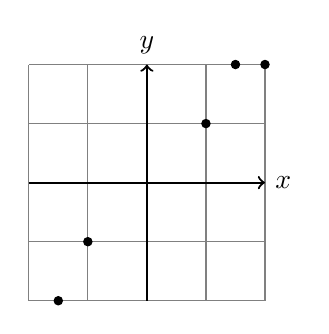
\begin{tikzpicture}[scale=0.75]
            \draw[gray] (-2,-2) grid (2,2); 
            \draw[->, thick]  (-2,0) -- (2,0)node [right] {$x$};
            \draw[->, thick]  (0,-2) -- (0,2)node [above] {$y$}; 
            \foreach \x/\y in {-1.5/-2,-1/-1,1/1,1.5/2,2/2} \filldraw (\x,\y) circle (.2em); 
    \end{tikzpicture}
    }
    \end{center}
    \end{minipage} 
    \onslide<4->{
    \vspace{12pt}
    \begin{center}
        Suppose we wanted to fit a straight line of the form $y = mx+b$ to our data. But how can we determine $m$ and $b$?  
    \end{center}
    }
\end{frame}


\begin{frame}{The Least-Squares Solution to a Linear System}
    \vspace{-6pt}
        \begin{center}
        \begin{tabular}{c|ccccc} 
            $ x$ & $-1.5$ & $-1$  & $1$ & $1.5$ & $2$
            \\ \hline 
            $ y$ & $-2$ & $-1$  & $1$ & $2$  & $2$
        \end{tabular}
    \end{center}
    Using the model $y=mx + b$, 
    
    \begin{minipage}{0.45\textwidth}
    \begin{align*}
        \onslide<2->{ m(-1.5) + b = -2 }  \\
        \onslide<3->{ m(-1) + b = -1 }  \\
        \onslide<4->{ m(1) + b = 1 } \\
        \onslide<5->{ m(1.5) + b = 2 } \\       
        \onslide<5->{ m(2) + b = 2 }     
    \end{align*}
    \end{minipage}    \begin{minipage}{0.45\textwidth}
    \onslide<6->{
    $$\Rightarrow \quad \spalignmat{-1.5 1;-1 1;1 1;1.5 1;2 1}\spalignmat{m; b}=\spalignmat{-2;-1;1;2;2}$$}
    \end{minipage}
    
    \vspace{2pt}
    \onslide<7->{We have a system of the form $A\vec x = \vec b$. There is no solution to our system, because there is no line that passes through all data points.} \onslide<8->{To find the line that \Emph{best} approximates our data we can use \Emph{least-squares}.}

\end{frame}






\begin{frame}{The Least-Squares Solution to a Linear System}

    \begin{center}\begin{tikzpicture} \node [mybox](box){\begin{minipage}{0.85\textwidth}
        Let $ A$ be an $ m \times n $ matrix. 
        A \Emph{least-squares solution to $ A \vec x = \vec b$} is \onslide<2->{ the solution $ \widehat x $ for which} \onslide<3->{ 
        \begin{equation*}
            \lVert \, \vec b - A \widehat x \, \rVert \leq \lVert \, \vec b - A  \vec x \, \rVert 
        \end{equation*}
        for all $\vec x\in \mathbb R ^{n}$.}
        \end{minipage}};\node[fancytitle, right=10pt] at (box.north west) {Definition:  Least-Squares Solution};
    \end{tikzpicture}\end{center}
    
    
    \onslide<4->{
    In other words, we want to identify the $\vec x$ that minimizes $\lVert \, \vec b - A  \vec x \, \rVert $, which we denote as $\widehat x$. 
    }
    
%    \begin{minipage}{.4\textwidth} 
%            \begin{tikzpicture}[scale=0.7]
%            \draw[gray] (0,0) grid (3,3); 
%            \draw[->]  (-.5,0) -- (3.5,0)  node [below] {$ x$}; \draw[->]  (0,-.5) -- (0,3.5) node [left] {$ y$}; 
%                        \foreach \x/\y in  {0/.9, 1/.2, 2/2.5 , 3/2.5}   
%            \draw [red,thick] (\x,\y) -- (\x,\x);
%            \draw[->,very thick, DarkBlue] (0,0) --  (3.5,3.5); 
%            \foreach \x/\y in  {0/.9, 1/.2, 2/2.5 , 3/2.5}  \filldraw (\x,\y) circle (.2em);  
%            \end{tikzpicture}
%        \end{minipage}\begin{minipage}{.5\textwidth} 
%            $\lVert \vec b - A \widehat x \rVert^2$ is the sum of squares of the red lines.
%    \end{minipage}

\end{frame}

\begin{frame}{A Geometric Interpretation}

    \vspace{-12pt}
    \begin{center}
        \tdplotsetmaincoords{74}{20}
        \begin{tikzpicture}[scale=2.4,
            axis/.style={->,black,-stealth}, 
            vectorY/.style={-stealth,DarkBlue,very thick},
            vectorH/.style={-stealth,black,very thick},
            vectorV/.style={-stealth,DarkRed,very thick},
            dsline/.style={black,dashed},
            perpline/.style={black, thin},
            tdplot_main_coords
            ]
        
            \coordinate (O) at (0,0,0);
            \coordinate (Y) at (1,0,1);
            \coordinate (H) at (1,0,0);        
            \coordinate (V) at (1.2,1.3,0);        
            \coordinate (C) at (-.3,-1,0);        
        
            % plane
            \filldraw[draw=DarkBlue!40,fill=DarkBlue!08,]          
            (-1,-1,0) -- (2,-1,0) -- (2,1.5,0) -- (-1,1.5,0)
            -- cycle;
            
            % draw vectors
            \draw[vectorY] (O) -- (Y) node[above]{$\vec b$};
            \draw[vectorH] (O) -- (H) node[below]{$A \widehat x$};
        
            % draw perpendicular symbols
            \draw[perpline] (0.85,0.0,0.15) -- (1.00,0.0,0.15);
            \draw[perpline] (0.85,0.0,0.15) -- (0.85,0.0,0.00);
        
            % dashed lines
            \draw[dsline] (Y) -- (H) ;
        
            % other labels
            \draw (C) node[above]{Col$(A)$};
            \draw (O) node[below]{$\vec 0$};
            
            \onslide<2->{
            \draw[vectorV] (O) -- (V) node[below]{$A \vec x$};
            \draw[dsline,DarkRed] (Y) -- (V) ;
            }
        \end{tikzpicture}
    
        The closest vector in $\Col A$ to $\vec b$ is $A\widehat x$. 

    \end{center}

%%  itemize
\begin{itemize}
\item<3->  If $ \vec b \in \operatorname {Col} A$, then  $ A\widehat x =\vec b $ is consistent. 

\item<4-> In general, we seek $ \widehat x $ so that $ A \widehat x $ is as close to $ \vec b$ as possible. 
\end{itemize}
\onslide<5->{We will need a process to identify $\widehat x$. }
%% itemize
\end{frame}



 \frame{\frametitle{Summary}

    \SummaryLine \vspace{4pt}
    \begin{itemize}\setlength{\itemsep}{8pt}

    \item constructing a linear system of equations based on a linear model of the form $y = mx + b$
    
    \item the least-squares problem for $A\vec x = \vec b$

    \end{itemize}
    
    \vspace{16pt}
    \pause 
    
    
}


